\section{Results} \label{sec:results}

The results of a grounded theory study, as the name of the method itself
suggests, are grounded on the collected data, so the hypotheses emerge from
data. A grounded theory should describe the key relationships between the
categories that compose it, i.e., a set of inter-related hypotheses~\cite{hoda2017becoming}.
We present the categories of our grounded theory
about DevOps adoption as a network of three categories of enablers (\cat{automation},
\cat{sharing} and \cat{transparency}) that are commonly used to develop the core category
``collaboration culture". Based on our understanding, implementing enablers to develop the collaboration
culture typically lead to concepts related to two categories of outcomes:
\cat{agility} and \cat{resilience}. Moreover, there are two categories that can be considered
both as enablers and as outcomes: \cat{continuous measurement} and \cat{quality assurance}.
In this section we describe the relationships between those categories, i.e.,
the hypotheses.

\subsection{How to Adopt DevOps?}

In Section~\ref{sec:introduction}, we present the question: is there any
straight-forward way to adopt DevOps? Here, we elaborate a response,
based on the analyses conducted as detailed in the previous section. The main
point which should be formulated is the construction of a \cat{collaboration
culture} between the software development and operations teams and 
related activities. According to our findins, the other categories, 
many of which are also present in other studies that have investigated DevOps, 
only make sense if the practices and
concepts related to them either contribute to the level of \cat{collaboration
culture} or lead to the expected consequences of a \cat{collaboration 
culture}. This understanding induces several hypothesis, as discussed in 
what follows. 

\textbf{H1:} \textit{There is a group of categories related to DevOps adoption
that only make sense if used to increase the \cat{collaboration culture} level. We
call this group of categories of \textbf{enablers}}. Therefore, there is no increase in collaboration 
levelin the situations 
where exist some degree of
automation to support (a) deployment activities, (b) infrastructure provisioning and management, 
and (c) monitoring activities, though this automation is maintained within a silo---where
only one team is able or responsible to understand, adapt or
evolve the automation. Consequently, the DevOps adoption has not advanced. The same is valid to the
other \emph{enabling} categories. That is, in the situations where 
\cat{transparency} and \cat{sharing} do not contribute to
the \cat{collaboration culture}, they do not contribute to DevOps adoption as a whole. Next
we present some examples of the underlying raw data that support H1. 

``Look, inside the operations sector there was some degree of automation. The guy
had stored in his own machine bash scripts that helped him when setting up a
server or when creating a new database instance. Nevertheless, there was no DevOps
because there was no intrinsic relationship of this automation to the
development process"---P11, DevOps Supervisor, Brazil.

``Keeping the culture alive remains a challenge to us, and it is very
important. Here in our company, for example, we have Tech Talks that are
monthly conversations that we have with the teams. The purpose of these Tech
Talks is to share knowledge about technologies and work processes increasing the
transparency of how everything works. We also have a Slack channel called
DevOps as Culture where we discuss things of DevOps culture. The idea is not to
let the culture die, we are always feeding it with something, because that is
the DevOps essence for us"---P12, Cloud Engineer, United States.

\textbf{H2:} \textit{There is a group of categories related to DevOps adoption
that don't contributes to increase of collaboration culture level, but that are
pointed out as DevOps adoption related, because they emerge as expected or
necessary consequence of the adoption. We call this group of categories of
\textbf{outcomes}}. In a first moment, the simple fact that a team is more
agile in delivering software, or more resilient in failure recovery, does not
contributes directly to bring operations tasks closer to development tasks.
But, the respondents of the interviews frequently cited the capacity of
continuously delivery software and the strongly resilient infrastructure as
part of their DevOps adoption process. As part of our

\textbf{H3:} \textit{The categories \textbf{Continuous Measurement} and \textbf{Quality Assurance} are related both to DevOps enabling capacity and to DevOps outcoming}. Measurement is cited as a typical responsibility of the operations team. At the same time that the sharing of this responsibility contributes to reduce the silo, it is also cited as a necessary consequence after DevOps adoption, because the context of agility with continuous delivery of software requires more caution, which is supplied by the concepts related to \textbf{continuous measurement} category. The same premise is valid to \textbf{quality assurance} category. At first glance \textbf{quality assurance} appears as one response to the context of agility in operations provided by DevOps adoption. But, the efforts in quality assurance of software products increase the confidence between the dev and ops teams developing the level of \textbf{collaboration culture}.

\subsection{DevOps Enablers}

DevOps enablers are exactly the means commonly used to increase the level of the collaboration culture in a DevOps adoption process. We have identified five categories of DevOps enablers:

\begin{itemize}
\item Automation;
\item Continuous Measurement*;
\item Quality Assurance*;
\item Sharing; and
\item Transparency.
\end{itemize}

\footnotesize * This category is also presented as outcome

\normalsize
\textbf{H4:} \textit{There is no precedence between enablers in a DevOps
adoption process}. We have perceived that the adoption process can follow a
path that prioritizes specific enablers, on the condition that the level of
collaboration culture increases. And there is no enabler with evidence that
can be more efficient to another in collaboration culture development. For
example, in 14 interviews \textbf{automation} was cited as a very important
enabler to adopt DevOps. But, some respondents ponder that considering
automation with greater importance than other parts can be a risk:

``I think that the expansion of collaboration between teams involved other
things, it was not just automation. There must be an alignment with the
business needs. (...) I think that DevOps made possible a broader understanding
of software production and we were realizing exactly that it is not about
automating everything. What we need is a broader understanding of that task.
Sometimes, we conclude that the task is not completely necessary and then we
solve the problem by changing procedures without the effort necessary to
automate it. So, I see with caution a supposed vision that automate things can
be the way to implement DevOps" - P7, Support Analyst, Brazil

``Despite of we actually use automation in a reasonable number of scenarios, we have been able to develop our culture significantly without automation and I think that you can reach a good DevOps level with little or even no automation" - P8, DevOps Engineer, Brazil.

That is, although automation is a very commonly used enabler, it is possible to
increase the level of collaboration culture without focus on automating. And
this premise is valid to the other enablers. Each enabler will be detailed in
the sequence of the paper.

\subsection{DevOps Outcomes}
DevOps outcomes is that group of categories doesn't produces primarily the
expected effect of a DevOps enabler, typically concepts that are expected as
consequences of an adoption of DevOps. We have identified four categories that
can work as DevOps outcomes:

\begin{itemize}
\item Agility;
\item Continuous Measurement*;
\item Quality Assurance*; and
\item Resilience.
\end{itemize}

\footnotesize * This category is also presented as enabler


\normalsize
One well succeeded DevOps adoption typically increases the potential of
agility, continuous measurement, quality assurance and resilience of a team.
But, in some cases this potential is not completely used due business
decisions. For example, one respondent has cited that at a first moment the
company don't allowed the continuous deployment of applications in production:

``We had conditions and security to continuously publish in production,
however, in the beginning the managers were afraid and decidec that the
publication would happen weekly" P9, IT Manager, Brazil

In this case, DevOps increased the level of agility of the company, but, this
potential was not totally tapped.

As well as enablers, each outcome will be detailed in the sequence of the paper.

Based on H1-H4 hypothesis, in Fig. 2 is presented a three step model of how to
adopt DevOps according with our proposal.

\begin{itemize}
\item \textbf{Step 1}: Understand and disseminate that the main point should be
the development of a collaboration culture between development and operations
team.
\item \textbf{Step 2}: Select and develop the most suitable enablers according
with the context of your company. The enablers are means commonly used to
develop the collaboration culture and its concepts.
\item \textbf{Step 3}: Check the outcomes to verify the alignment of your
adoption with industrial practice and explore them according to the need of
your company.
\end{itemize}

\begin{figure*}
  \centering
    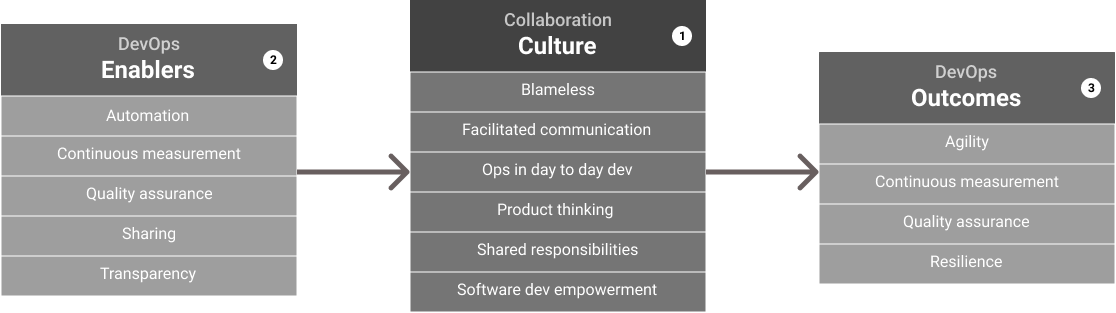
\includegraphics[width=14.26cm,height=4cm,natwidth=1116,natheight=313]{model.png}
    \caption{DevOps Adoption Model}
    \label{fig2}
\end{figure*}
